\documentclass[../main.tex]{subfiles}


\begin{document}

\section{Markovian Dynamics of the Junction Point $r_j$?}

If we describe the configurations of our copolymers by their complete set of segment positions we get true continuous time markovian dynamics.
This is due to the fact that we don't have any "hidden" variables and as such the future time evolution of the system depends only on the configuration of the current state.
Therefore -- as long as we ensure detailed balance -- we get the characteristic decay of the current configuration over some relaxation time $\tau_r$ that is connected to the largest eigenvalue of the transfer matrix.
\par

As we have seen, the junction point can be used as a reaction coordinate that characterizes the escape of the copolymer from the micelle.
We can therefore ask ourselves if it would be sufficient to only simulate the reaction coordinate with a detailed balance algorithm to obtain correct dynamics.
This would be a severe saving in computational resources and would allow us to study the system much more thoroughly.
Unfortunately this is not the case.
\par

If we considered the system's configuration to consist only of the junction point, we would discard the information of the state that corresponds to the sub chains.
The problem is easy to spot if one considers that the value of the junction point is symmetric under exchange of the sub chains.
Obviously the exchanged sub chains have to lead to different dynamics in the external field.
Therefore the future evolution of the system would not only be conditioned on the current configuration and the dynamics are not markovian.
\par

\section{Forward Flux Sampling - Transition Rates}

\begin{figure}[htpb]
    \centering
    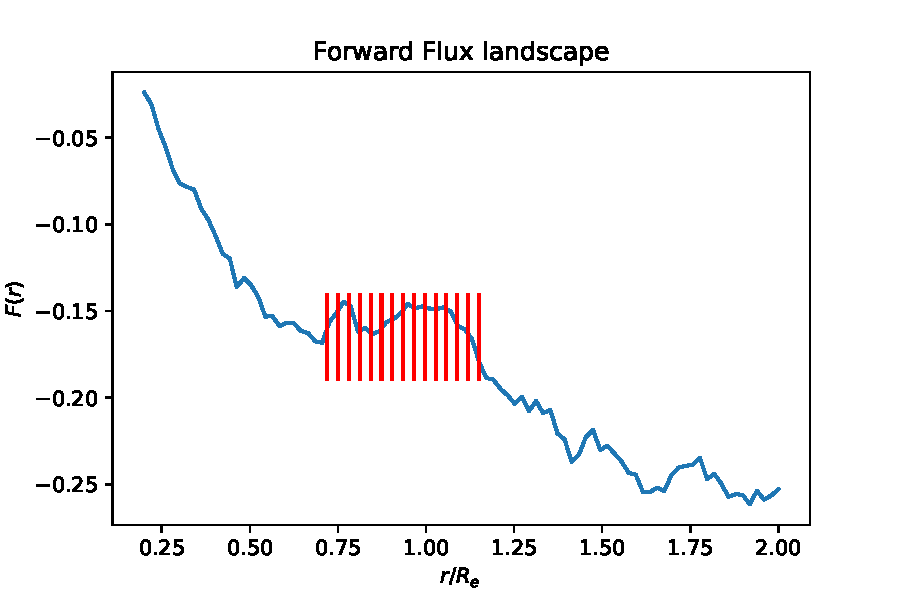
\includegraphics[width=0.8\textwidth]{../figures/ex2_forward_flux_landscape.pdf}
    \caption{Free Energy profile from Figure \ref{fig:ex1_free_energy_profile} but with the chosen Forward Flux interfaces shown as red vertical lines.}
    \label{fig:ex2_forward_flux_landscape}
\end{figure}

To calculate the transition rate of a single copolymer escaping the micelle we can use Forward Flux sampling.
Firstly we need to find a good way to define interfaces along the rise of the barrier.
We choose to use barriers in distances of around $\SI{.4}{\charenergy}$.
Then we fit a linear function to the rise and choose barriers in equal distances along the reaction coordinate such that the largest distance in the Free Energy is $\SI{.4}{\charenergy}$.
In Figure \ref{fig:ex2_forward_flux_landscape} the interfaces are embedded into the Free Energy landscape.
\par

The transition rate can thus be calculated as the product of the forward transition rates from one interface to the next.
The calculated value is $\eta = \SI{4+-1e-6}{\per\mcstep}$.

\section{Kramers Rate}

\begin{figure}[htpb]
    \centering
    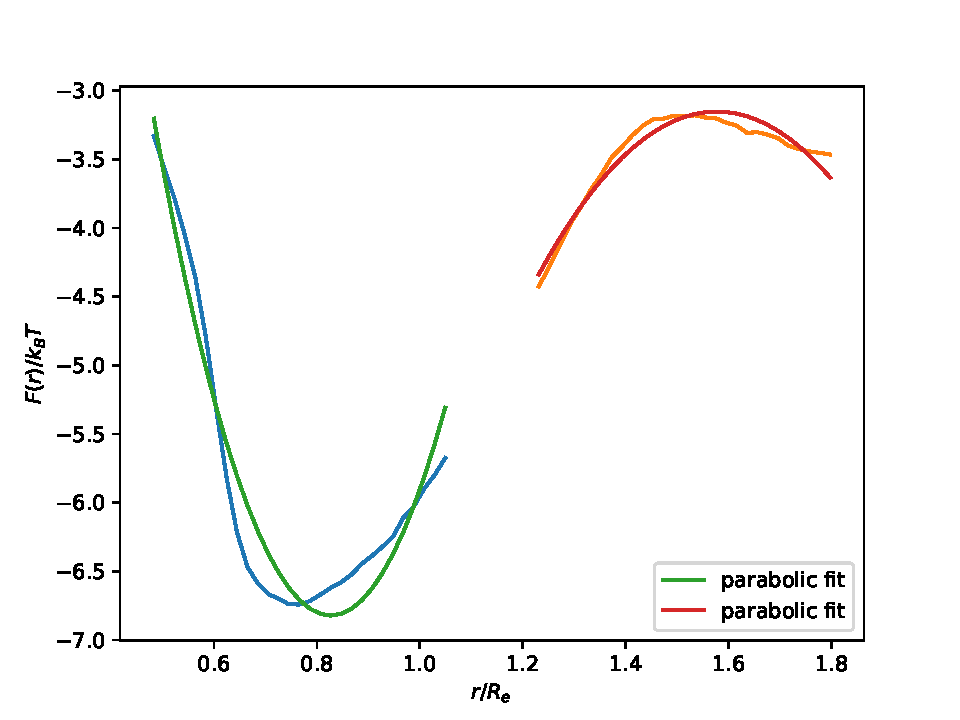
\includegraphics[width=0.8\textwidth]{../figures/ex2_parabolic_fit.pdf}
    \caption{
        Again plotted the same Free Energy Landscape used like in Figure \ref{fig:ex1_free_energy_profile} but only the parts that were used to fit quadratic functions to the extrema are filled in.
    }
    \label{fig:ex2_parabolic_fit}
\end{figure}

Alternatively to the Forward Flux sampling process we can also estimate the transition rate via the Kramers rate.
The formula for the Kramers rate given is 
\[
    \eta_k = \frac{D}{\pi \unit{\charenergy}} 
    \sqrt{F^{\prime \prime}_{ \text{max} } F^{\prime\prime}_{ \text{min} } } \exp( - \frac{\Delta F}{\unit{\charenergy}} )  
.\] 
Here $F^{\prime \prime}_{ \text{max} }$ and $F^{\prime \prime}_{ \text{min} }$ are the second derivative of the Free Energy at the maximum or minimum respectively.
To calculate accurate values for these we can fit a parabola to an selected environment around the minimum.
From these calculations and using our results for the diffusion constant $D$ and $\Delta f$ we obtain $\eta_k = \SI{1.35e-6}{\per\mcstep}$.


\ifSubfilesClassLoaded{
	% if it's compiled alone
}{
	% if it's compiled in the main file
}
\end{document}

